\section{Related work}
\label{sec:related_work}
%
Previous work on exploring volumetric data to address occlusion issues can be divided into occlusion management techniques and lenses-and-deformation techniques. We next discuss these and also point out existing limitations from the perspective of the four requirements (R1,$\ldots$,R4) introduced in Sec.~1.

\begin{figure*}[htbp]
\centering
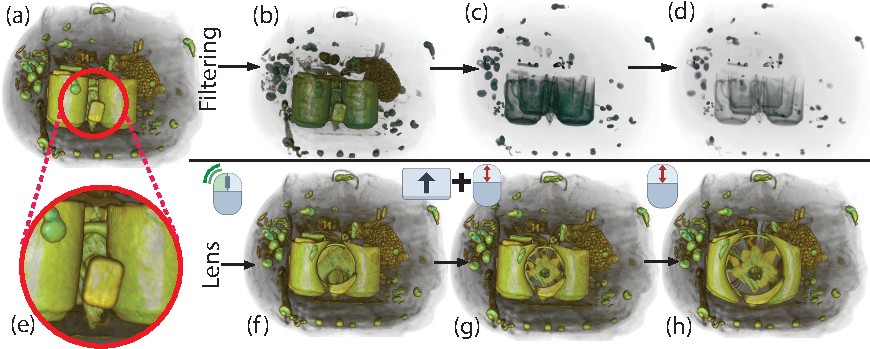
\includegraphics [width=0.9\textwidth]{shuriken.eps}
\vspace{-0.15cm}
\caption{(a-c) A baggage scan is viewed from different angles. In view (c), a suspicious sharp object is spotted between a set of mugs. (d-f) Filtering densities using a classical 1D opacity transfer function removes progressively more of the occluders (mugs), but also the target. (g) The user applies the lens on the target object (double-click). An animation starts opening the lens, rays are gathered to pass through occluders. Halfway the animation, the object is magnified, but only the area close to the lens is visible. (h) The fish-eye field of view at the end of the animation scatters rays to fully show the target. (i) The lens is increased to magnify the target (mouse scroll).}
\label{f:baggage_lens}
\end{figure*}
\vspace{-0.15cm}


\subsection{Occlusion management}
%
Many approaches for occlusion management have been proposed\,\cite{4483791}. Multiple viewports can be used to see the data from different perspectives\,\cite{WangBaldonado:2000:GUM:345513.345271}. This does not help when the target is strongly occluded from \emph{all} possible viewpoints (R4). Virtual X-ray methods make targets visible by turning occluders invisible or half-transparent\,\cite{Burns:2008:ACC:1457515.1409107}. Kruger et al.\,\cite{4015450} proposed ClearView, an interactive technique that enables focusing on particular areas in the data while preserving context information without visual clutter by modulating transparency. Correa and Ma\,\cite{5416704} proposed visibility-driven transfer functions (TFs) to maximize the visibility of selected data-intervals. Designing good TFs is still challenging and time-consuming (R2) in general: For instance, in baggage inspection, a dissimulation strategy is to hide a threat among same-density objects, so TF editing cannot easily remove occluders but keep the target (R4)\,\cite{7819413}. Similar situations occur when aiming to de-occlude a tumor from surrounding similar-density tissue in medical scans\,\cite{CGF:CGF12927}. 
Rezk-Salama and Kolb\,\cite{CGF:CGF979} also considered the voxels' occurrence on the cast ray, besides their densities and positions. Hurter et al.\,\cite{moleview,6787171} proposed several lens techniques to remove occluders by deforming (pushing them away) in a focus area, applicable to 2D images, multivariate volumes, and trail sets. Such techniques specify occluders based on data value-ranges, thus share limitations with ClearView and related techniques. Li et al.\,\cite{Li:2012:LVV:2425296.2425325} proposed a system for luggage virtual unpacking where targets are cleared by interactively moving away occluders. This however severely alters the \emph{context} where occluders occur (R3), by altering or removing potentially important information, \emph{e.g.}, relative position and connectivity -- a clear limitation in this but also other, \emph{e.g.} medical, contexts. Recently, an interactive visualization system was proposed for volumetric data exploration via direct voxel manipulation\,\cite{7819413}. Extending such approaches in a DVR setting to more complex deformations or changes of the data in focus is computationally challenging (R1).

\vspace{-0.15cm}
\subsection{Lenses and deformations}
%
An interactive lens is a lightweight tool to solve localized visualization problems by temporarily altering a selected part of the visual data representation\,\cite{CGF:CGF12871}. In other words, a lens is a parameterizable selection that alters a base visualization, and as such can effectively provide focus-and-context (F+C) solutions to volumetric data occlusion (R2). Parametrizable lens properties include position, shape, appearance, size, orientation, and selection of included data (focus). The lens \emph{shape} is usually chosen to fulfill the requirements of the application and is strongly linked to the lens function. Most lenses are circular\,\cite{1648236} or rectangular\,\cite{Kincaid:2010:SFA:1907651.1907963}, a design that we also choose. The JellyLens\,\cite{Pindat:2012:JCA:2380116.2380150} and smart lenses\,\cite{Thiede2008}, adapt their shape automatically to the focus data. Modifying the lens \emph{position} and/or \emph{size} sets its focus on a different part of the data based on the user's interest. Position and size can be changed automatically to guide the user toward interesting events in the data\,\cite{Tominski:2011:ECU:2336207.2336211} or guide the exploration path along interesting events\,\cite{Alvina:2014:RER:2598153.2598200}. Our lens updates automatically its properties once a target has been selected. This allows a smooth transition towards an unobstructed and magnified area of interest.

Lenses for DVR face spatial selection and occlusion challenges. The Magic Lens\,\cite{1532818} addresses these by rendering occlusions with lower opacity and magnifying volumetric pre-computed features interactively or automatically in a pre-segmented dataset. This however does not provide an (interactive) way to deal with similar-density occluders and targets (R1,R4). Besides interactively magnifying targets, our lens frees them from occlusion and allows local modification of the viewpoint, lighting, and TF, to offer many exploration perspectives. The GlyphLens\,\cite{7539643} removes occluding glyphs by pulling them aside through animation. While effective, this technique covers only 3D glyph-based volumetric visualizations. Lenses can create discontinuities between their inner part and the rest of the volume. Deformation can be a solution to this discontinuity issue.

Hsu et al.\,\cite{Hsu:2011:RFM:2070781.2024165} increase deformation flexibility by using non-linearly sampled rays to smoothly project objects at multiple levels of detail onto a single image. This requires significant computational effort to render a single image from features of interest at different scales (R2). Bruckner and Gr{\"o}ller~\cite{4015467} proposed exploded views for volume data by partitioning the volume into several segments. Correa et al.\,\cite{Correa:2007:IDD:1313046.1313163} allow users to physically manipulate the geometry of a data object. McGuffin et al.\,\cite{1250400} performed deformations using peeling to see hidden parts of the data. In general, these techniques have the issue of removing potentially important contextual information surrounding the target when trying to solve the local occlusion (R3).

Deformations can reveal predefined features in the data by taking into account a precomputed segmentation. Tong et al. proposed a deforming lens which moves streamlines to observe the inner part of streamline bundles\,\cite{7332955}. Other techniques performed deformations using surgical metaphors\,\cite{4069230,Correa:2006:FAV:1187627.1187827} to show hidden parts of a volume. Such techniques do not offer tools for local manipulation of the viewpoint that allows seeing a target under multiple perspectives while keeping the global context (R3). To this end, our lens proposes an interactive volume deformation based on GPU accelerated ray-casting to free a designated target from local occlusion while keeping the global context.

\vspace{-0.09cm}
\subsection{Detailed contributions}
%

\noindent\textbf{ALEX: Add summary table here.}

Summarizing the above discussion on the requirements and related work on occlusion management, we propose a new technique which combines high-quality DVR with a fast, versatile, and easy to use, lens to support the interactive exploration of occluded data in volumes. In the classification of view deformations by Carpendale \emph{et al.}\,\cite{595268}, we use a nonlinear radial distortion through an interactive lens to remove occluding items and keep the global context while magnifying a partially occluded item. Related to volumetric lens techniques, we frame our contribution as follows:
 
\begin{itemize}
\item  we propose an interactive deforming lens that magnifies and pushes aside occluding objects located in front of a designated focal point which meets the four requirements in Sec. 1;
\item the combination of flexible and real-time interactive changing of the focal point, custom bent rays used for DVR, lens deformation, and shading and transfer function in the focus area allow us to provide \emph{on the fly} a range of perspectives of the targets, without having to change the viewpoint or manipulate complex parameters in multiple linked views.
\end{itemize}


